\documentclass[11pt,aspectratio=169]{beamer}
%%%%%%%%% GENERAL PACKAGES
%\usepackage[dvipsnames]{xcolor}
%\usepackage{pdfpages}
%\usetheme[progressbar=frametitle]{metropolis}
%\setbeamercolor{background canvas}{bg=white}
%\usepackage{appendixnumberbeamer}
%\usepackage{booktabs}
%\usepackage[scale=2]{ccicons}
%\usepackage{pgfplots}
%\usepgfplotslibrary{dateplot}
%\usepackage{xspace}
%\newcommand{\themename}{\textbf{\textsc{metropolis}}\xspace}
%\usepackage[absolute,overlay]{textpos}






%%%%%%%%% COLOR THEME

% Define some colors:
\definecolor{DarkFern}{HTML}{407428}
\definecolor{DarkCharcoal}{HTML}{4D4944}
\definecolor{AlertColor}{RGB}{89,124,158}
\definecolor{HighLight}{RGB}{96,95,134}
\definecolor{Important}{RGB}{234,122,133}
\definecolor{Yellow}{HTML}{00539C}
\colorlet{Fern}{DarkFern!85!white}
\colorlet{Charcoal}{DarkCharcoal!85!white}
\colorlet{LightCharcoal}{Charcoal!50!white}
\colorlet{HighLight2}{AlertColor}
\colorlet{DarkRed}{red!70!black}
\colorlet{DarkBlue}{blue!70!black}
\colorlet{DarkGreen}{green!70!black}
\definecolor{RoyalBlue}{HTML}{00539C}
\definecolor{Peach}{HTML}{EEA47F}
\definecolor{ForestGreen}{HTML}{2C5F2D}
\definecolor{MossGreen}{HTML}{E8FCC9}
\definecolor{SeaGreen}{HTML}{2E8B57}
% Use the colors:
\setbeamercolor{title}{fg=Fern}
\setbeamercolor{frametitle}{fg=MossGreen,bg=ForestGreen}
\setbeamercolor{normal text}{fg=Charcoal!70!black}
\setbeamercolor{block title}{fg=black,bg=Fern!25!white}
\setbeamercolor{block body}{fg=black,bg=Fern!10!white}
\setbeamercolor{block title alerted}{fg=black,bg=DarkRed!25!white}
\setbeamercolor{block body alerted}{fg=black,bg=DarkRed!10!white}
\setbeamercolor{alerted text}{fg=DarkRed}
\setbeamercolor{itemize item}{fg=Charcoal}



%%%%%%%%% OTHER COMMANDS
\newcommand{\indep}{\perp\!\!\! \perp}
\newcommand{\comment}[1]{}
\newcommand{\bs}{\boldsymbol}
\newcommand{\tr}{\text{trace}}
\newcommand{\sgn}{{\rm sgn}}
\def\T{\top}
%\newcommand{\det}{\text{det}}
\newcommand{\var}{\mathrm{var}}
\newcommand{\cC}{{\cal C}}
\renewcommand{\d}{{\rm d}}
\newcommand{\cG}{{\cal G}}
\newcommand{\cV}{{\cal V}}
\newcommand{\cE}{{\cal E}}
\newcommand{\cM}{{\cal M}}
\newcommand{\cP}{{\cal P}}
\newcommand{\cX}{{\cal X}}
\newcommand{\cY}{{\cal Y}}
\newcommand{\X}{\mathbf{X}}
\newcommand{\Y}{\mathbf{Y}}
\newcommand{\x}{\mathbf{x}}
\newcommand{\y}{\mathbf{y}}
\newcommand{\z}{\mathbf{z}}

\newcommand{\argmin}{\operatornamewithlimits{argmin}}
\newcommand{\eps}{\varepsilon}
\newcommand{\<}{\langle}
\renewcommand{\>}{\rangle}


%

\setbeamertemplate{navigation symbols}{}
\setbeamertemplate{footline}[text line]{%
    \hfill\strut{%
        \scriptsize\sf\color{black!60}%
        \quad\insertframenumber/\inserttotalframenumber
    }
    %\hfill
    }


\usenavigationsymbolstemplate{}
\setbeamersize{text margin left=.2cm,text margin right=.2cm} 
\addtobeamertemplate{frametitle}{}{\vspace{-1.2mm}}
\setbeamertemplate{itemize item}{$\bullet$}

\setbeamertemplate{itemize subitem}{\tiny\raise1.5pt\hbox{\donotcoloroutermaths$\blacktriangleright$}}
\setbeamertemplate{itemize subsubitem}{\tiny\raise1.5pt\hbox{\donotcoloroutermaths$\blacktriangleright$}}
\setbeamertemplate{enumerate item}{\insertenumlabel.}
\setbeamertemplate{enumerate subitem}{\insertenumlabel.\insertsubenumlabel}
\setbeamertemplate{enumerate subsubitem}{\insertenumlabel.\insertsubenumlabel.\insertsubsubenumlabel}
\setbeamertemplate{enumerate mini template}{\insertenumlabel}






\newcommand{\TODO}[1]{{\color{red}{[TODO: #1]}}}


\newcommand{\R}{\mathbb R}
\newcommand{\E}{\mathbb E}
\renewcommand{\P}{\mathbb P}


\DeclareMathOperator*{\cov}{cov}


\newsavebox{\zerobox}
\newenvironment{nospace}
{\par\edef\theprevdepth{\the\prevdepth}\nointerlineskip
  \setbox\zerobox=\vtop to 0pt\bgroup
  \hrule height0pt\kern\dimexpr\baselineskip-\topskip\relax
}
{\par\vss\egroup\ht\zerobox=0pt \wd\zerobox=0pt \dp\zerobox=0pt
  \box\zerobox}

\usepackage{soul}
\makeatletter
\let\HL\hl
\renewcommand\hl{%
  \let\set@color\beamerorig@set@color
  \let\reset@color\beamerorig@reset@color
  \HL}
  \makeatother



%\usecolortheme{whale}

\title[Calculus and Linear Algebra]{Lecture 3: Calculus and Linear Algebra}
\author[Piotr Zwiernik, Barcelona School of Economics]{Piotr Zwiernik \\ $\;$\\
Mathematics Brush-up\\ $\;$\\ $\;$\\

\includegraphics[width=1.5in]{img/bse.png}  
}
\date{}

%\beamerdefaultoverlayspecification{<+->}

\begin{document}
\begin{frame}
\titlepage
\end{frame}


\begin{frame}
\frametitle{Chapter 7: Systems of Linear equations}
\begin{small}
Many problems in economics can be modeled as \textcolor{blue}{system of linear equations}.
\vskip 12pt
In previous chapters we have already encountered systems of linear equations.
\vskip 12pt
In this chapter, we consider some basic properties of such systems and discuss \textcolor{blue}{general solution procedures}.

\vskip 12pt
\textcolor{blue}{Read}  Chapter 8 of Werner-Sotskov and Chapter 7 of Simon-Blume
\vskip 12pt
 \textcolor{blue}{Exercises:} 8.5, 8.6, 8.8 (Werner-Sotskov)


\end{small}
\end{frame}


\begin{frame}
\frametitle{Systems of linear equations}
\begin{small}
 Let $A$ be a $m \times n$ matrix, ${\bf x}=(x_1, \ldots, x_n)$ a vector (unknown) in $\R^n$ and ${\bf b}$ a vector (given) in $\R^m$. Then the equation $$A {\bf x}={\bf b}$$ is a \textcolor{blue}{system of $m$ linear equations and $n$ variables}.
\vskip 12pt
In vector representation, the system writes as 
$$
\sum_{j=1}^n x_j {\bf a_j}={\bf b},
$$
where ${\bf a_1},\dots, {\bf a_n}$ are the column vectors of  $A$.
\vskip 12pt
If ${\bf b}={\bf 0}$ the system is called \textcolor{blue}{homogeneous}, otherwise is called \textcolor{blue}{inhomogeneous}.
An \textcolor{blue}{inhomogeneous} system can have  no solution (inconsistent system) or at least one solution  (consistent system).
An \textcolor{blue}{homogeneous} system has always the solution ${\bf x}={\bf 0}$.

\end{small}
\end{frame}


\begin{frame}
\frametitle{Existence and uniqueness of a solution}
\begin{small}
\textcolor{blue}{Theorem:} Let $A$ be a $m \times n$ matrix. 
The \textcolor{blue}{maximum} number of linearly independent \textcolor{blue}{column} vectors of $A$ coincides with the maximum number of linearly independent \textcolor{blue}{row} vectors. 
\vskip 10pt
This number is called the \textcolor{blue}{rank} of $A$, and denoted $r(A)$. 
\vskip 10pt
\textcolor{blue}{Theorem:} The rank of a matrix $A$ equals to the largest order of a \textcolor{blue}{minor} of $A$ that is \textcolor{blue}{different from zero}. Recall that a minor is the determinant of a square submatrix of $A$.
\vskip 10pt
\textcolor{blue}{Example:}
\begin{equation*}
A=\begin{pmatrix}
1 & 2 & 0\\
4 & 6 & 2 \\
3 & 2 & 4
\end{pmatrix}
\end{equation*}
Since $\vert A \vert=0$, $r(A) \leq 2$. Since $\vert A_{33} \vert=-2$, $r(A)=2$.

\begin{tiny} Observe that $2{\bf a_1}-{\bf a_2}={\bf a_3}$ but none of the  columns is a multiple of the other, so 
the  families $\{{\bf a_1}, {\bf a_2}\}$, $\{{\bf a_1}, {\bf a_3}\}$ and $\{{\bf a_2}, {\bf a_3}\}$  are l.i. and span the same subspace.\end{tiny}



\end{small}
\end{frame}

\begin{frame}
\frametitle{Computing the rank with Gaussian elimination}
\begin{small}
The rank of a matrix does not change either if we apply elementary columns or row operations to the matrix.

 \textcolor{blue}{Example:}
\begin{equation*}
A=\begin{pmatrix}
1 & 2 & 0\\
4 & 6 & 2 \\
3 & 2 & 4 \end{pmatrix} \sim \begin{pmatrix}
1 & 2 & 0\\
0 & -2 & 2 \\
0 & -4 & 4
\end{pmatrix} \sim 
\begin{pmatrix}
1 & 2 & 0\\
0 & -2 & 2 \\
0 & 0 & 0
\end{pmatrix}
\end{equation*}
Since the  third row has no pivot the columns are  l.d. and since the matrix has  2 pivots the  rank  is 2. \begin{tiny}The pivot is the first non-zero value of a non-zero row after reducing the matrix with Gaussian elimination. The number of pivots equals the rank. \end{tiny}

To find a relation between columns we need to solve the homogeneous system
\begin{equation*}
\begin{split}
\lambda_1+2\lambda_2&=0 \\
-\lambda_2+\lambda_3&=0 
\end{split}
\end{equation*}
The solution is $(-2\lambda_3, \lambda_3, \lambda_3)$. If for example $\lambda_3=1$, we obtain  the relation
$$
-2 {\bf a_1}+{\bf a_2}+{\bf a_3}=0.
$$


\end{small}
\end{frame}

\begin{frame}
\frametitle{Existence and uniqueness of a solution}
\begin{small}
 We define the \textcolor{blue}{augmented matrix} of $A$ the $m \times (n+1)$ matrix whose columns are the columns of $A$ plus the vector ${\bf b}$. We denote it by $A_{{\bf b}}$.
\vskip 10pt
\textcolor{blue}{Remark:} Either $r(A_{{\bf b}})=r(A)$, either $r(A_{{\bf b}})=r(A)+1$.
\vskip 10pt
 \textcolor{blue}{Theorem:} A linear system $A {\bf x}={\bf b}$ is \textcolor{blue}{consistent} (at least one solution) if and only if $r(A_{{\bf b}})=r(A)$. \begin{tiny} (which is equivalent to ${\bf b}\in \text{Span}\{ {\bf a_1},\ldots,{\bf a_n}\}$)\end{tiny}
\vskip 12pt
 \textcolor{blue}{Theorem:} Consider a consistent linear system $A {\bf x}={\bf b}$ , where $A$ is $m \times n$.
\begin{enumerate}
\item If $r(A_{{\bf b}})=r(A)=n$, then the solution is \textcolor{blue}{unique}.
\vskip 12pt
\item If $r(A_{{\bf b}})=r(A)<n$, then there exist \textcolor{blue}{infinite} many solutions and we need to choose $n-r(A)$ variables \textcolor{blue}{free}.
\end{enumerate}



\end{small}
\end{frame}\begin{frame}
\frametitle{Elementary transformation; solution procedures}
\begin{small}
\textcolor{blue}{Theorem:} The set of solution does not change if we apply one of the \textcolor{blue}{elementary row operations} to the matrix $A_{{\bf b}}$.

\vskip 12pt

\textcolor{blue}{Theorem (Gauss elimination):} Applying elementary row operations  
to the augmented matrix any system can be transformed into a triangular system.
\vskip 12pt
\textcolor{blue}{Example:}
\begin{equation*}
\begin{split}
x_1+x_2+x_3&=3 \qquad \qquad \qquad x_1+x_2+x_3=3 \\
x_1-x_2+2x_3&=2 \qquad \Longleftrightarrow\qquad -2x_2+x_3=-1\\
4x_1+6x_2-x_3&=9 \qquad \qquad \qquad -4x_3=-4
\end{split}
\end{equation*}
\begin{tiny}
We have done the row operations: $r_2-r_1$, $r_3-4r_1$ and $r_3+r_2$. 
\vskip 10pt
We have $r(A_{{\bf b}})=r(A)=3$ (3 pivots) so the solution is unique.

Both systems have  the unique solution $(1,1,1)$. \end{tiny}


\end{small}
\end{frame}

\begin{frame}
\frametitle{Example}
\begin{small}
Consider the \textcolor{blue}{homogeneous} system of equations
\begin{equation*}
\begin{split}
a+b+c+d+e+f&=0   \\
2a+2b+2c+2d-e-f&=0 \\
3a+3b-c-d-e-f&=0 
\end{split}
\end{equation*}

By Gaussian elimination, we obtain
\begin{equation*}
A\sim\begin{pmatrix}
1&1&0&0&0&0\\
0&0&1&1&0&0\\
0&0&0&0&1&1 \end{pmatrix} 
\end{equation*}
\begin{tiny}This matrix has 3 pivots so  the rank is 3, so  the set of solutions is a subspace of dimension $6-r(A)=3$.\end{tiny}

This corresponds to the homogeneous system $a+b=0$, $c+d=0$, $e+f=0$. We choose \textcolor{blue}{3 variables free} and we obtain the general solution
$$
(a, -a, c, -c, e, -e).
$$
 \begin{tiny}A basis of the subspace of solutions is $\{(1,-1,0,0,0,0),(0,0,1,-1,0,0), (0,0,0,0,1,-1)  \}$.
 \end{tiny}



\end{small}
\end{frame}

\begin{frame}
\frametitle{General solution}
\begin{small}
 \textcolor{blue}{Theorem:} Every solution to the system $A {\bf x}={\bf b}$ can be written as 
$${\bf x}={\bf x}_h+{\bf x}_p,$$where ${\bf x}_h$ is the \textcolor{blue}{general solution} to the homogeneous system
$A{\bf x}={\bf 0}$, and ${\bf x}_p$ is a \textcolor{blue}{particular solution} of $A{\bf x}={\bf b}$.
\vskip 10pt
\textcolor{blue}{Corollary:} If $A{\bf x}={\bf b}$ is consistent, then the number of solutions is the same as the number of solutions to $A{\bf x}={\bf 0}$.
\vskip 10pt
 \textcolor{blue}{Example:}
\begin{equation*}
\begin{split}
x_1+x_2+x_3&=1 \qquad \qquad \qquad  \\
x_1+x_2+x_3&=1 \qquad \Longleftrightarrow \qquad x_1+x_2+x_3=1\\
x_1+x_2+x_3&=1 \qquad \qquad \qquad 
\end{split}
\end{equation*}
\begin{tiny}The matrix has 1 pivot so $r(A)=r(A_{{\bf b}})=1$, so we choose 2 variables free. \end{tiny}
General solution: $$\begin{pmatrix}
x_1\\
x_2\\
x_3
\end{pmatrix}=\lambda_1 \begin{pmatrix}
-1\\
1\\
0
\end{pmatrix}
+\lambda_2 \begin{pmatrix}
-1\\
0\\
1
\end{pmatrix}+\begin{pmatrix}
1\\
0\\
0
\end{pmatrix}, \quad \lambda_1, \lambda_2 \in \R$$


\end{small}
\end{frame}

\begin{frame}
\frametitle{Examples}
\begin{small}
\begin{enumerate}

\item Consider the matrix \begin{equation*}
A=\begin{pmatrix}
1 & 2 & 0\\
4 & 6 & 2 \\
3 & 2 & 4
\end{pmatrix}
\end{equation*}
We have already seen that $r(A)=2$, thus the solution to the system $A{\bf x}={\bf 0}$ has dimension $3-r(A)=1$ and is the line $\{\lambda (-2,1,1), \lambda \in \R\}$.

\item Consider the system of equations
\begin{equation*}
\begin{split}
x_1+x_2+x_3&=-1 \\
x_1+2x_2+4x_3&=2 
\end{split}
\end{equation*}
By Gauss elimination we obtain the equivalent system \begin{equation*}
\begin{split}
x_1+x_2+x_3&=-1 \\
x_2+3x_3&=3\\
\end{split}
\end{equation*}
Therefore $r(A)=r(A_{{\bf b}})=2$ and we choose $1$  variable  free.
The solution is $\{\lambda (2, -3, 1)+(-4,3, 0), \lambda \in \R\}$.
\end{enumerate}

\end{small}
\end{frame}

\begin{frame}
\frametitle{Example}
\begin{small}
We want to compute the  \textcolor{blue}{canonical basis} of  the  subspace spanned by the vectors
\begin{equation*}
{\bf v_1}=\begin{pmatrix}
2 \\
-1  \\
0 
\end{pmatrix}\qquad
{\bf v_2}=\begin{pmatrix}
3 \\
0  \\
-1 
\end{pmatrix}\qquad
{\bf v_3}=\begin{pmatrix}
0 \\
3  \\
-2 
\end{pmatrix}
\end{equation*}

We do  Gaussian \textcolor{blue}{row} elimination to the \textcolor{blue}{transpose matrix}
\begin{equation*}
\begin{pmatrix}
2&-1&0 \\
3  &0&-1\\
0 &3&-2
\end{pmatrix}\sim
\begin{pmatrix}
1&0&-1/3 \\
0  &1&-2/3\\
0 &0&0
\end{pmatrix}
\end{equation*}

\begin{tiny} If  we  de not consider the transpose matrix then  we need to do column operations.

Doing row operations and solving  the homogeneous system we obtain the relation
$3 {\bf v_1}-2{\bf v_2}+{\bf  v_3}=0$\end{tiny}
\vskip 10pt
The canonical basis is $\{(1,0,-1/3), (0,1,-2/3)\}$.

\begin{tiny} Other bases are $\{\vec{v}_1, \vec{v}_2\}$, $\{\vec{v}_1, \vec{v}_3\}$ and $\{\vec{v}_2, \vec{v}_3\}$.
\end{tiny}

\end{small}
\end{frame}



\begin{frame}
\frametitle{Chapter 8: Eigenvalue problems and quadratic forms}
\begin{small}
\textcolor{blue}{Eigenvalue problems} and \textcolor{blue}{quadratic forms} are useful for deciding whether a function has an extreme point or for solving certain types of differential equations.
\vskip 12pt
 \textcolor{blue}{Eigenvalues} often arise in economic problems dealing with processes of proportionate growth or decline.
\vskip 12pt
\textcolor{blue}{Quadratic forms} play an important role in optimization problems of functions of several variables. 
\vskip 12pt
\textcolor{blue}{Read}  Chapter 10 of Werner-Sotskov and (optional) Chapter 7 of Simon-Blume

\vskip 12pt
\textcolor{blue}{Exercises:} 10.2, 10.5 A,B,C, 10.6 a), b) (Werner-Sotskov)


\end{small}
\end{frame}

\begin{frame}
\frametitle{Eigenvalues and eigenvectors: Economic example}
\begin{small}
Let $x_t^M$ and $x_t^W$ be the number of men and women in some population at time $t$. 
\vskip 10pt
We assume they satisfy the relation
\begin{equation*}
\begin{pmatrix}
x^M_{t+1} \\
x_{t+1}^W
\end{pmatrix}
=\begin{pmatrix}
0.8 & 0.4  \\
0.3 & 0.9
\end{pmatrix}
\begin{pmatrix}
x^M_{t} \\
x_{t}^W
\end{pmatrix}
\end{equation*}

Moreover, we assume the ratio of men and woman is constant over time, that is,
 \begin{equation*}
\begin{pmatrix}
x^M_{t+1} \\
x_{t+1}^W
\end{pmatrix}
=\lambda
\begin{pmatrix}
x^M_{t} \\
x_{t}^W
\end{pmatrix}
\end{equation*}
\vskip 12pt
\textcolor{blue}{Question:} Do $\lambda$ and ${\bf x_t}'=(x_t^M, x_t^W)$ satisfying the above equations exist ? 

\end{small}
\end{frame}

\begin{frame}
\frametitle{Eigenvalues and eigenvectors }
\begin{small}
Let $A$ be an $n \times n$ matrix. A scalar $\lambda \in \R$ is called an \textcolor{blue}{eigenvalue} of $A$ if there exists ${\bf x} \in \R^n$, ${\bf x} \neq {\bf 0}$ solution to the equation
$$
A {\bf x}=\lambda {\bf x}.
$$
Then ${\bf x}$ is called an \textcolor{blue}{eigenvector of $A$ with eigenvalue $\lambda$}.
\vskip 12pt
Intuitively the linear transformation given by $A$ transforms ${\bf x}$ into a co-linear  vector.
\vskip 12pt
By definition the vector ${\bf 0}$ is never considered an eigenvector!

\vskip 12pt
The example above corresponds to finding the \textcolor{blue}{eigenvalues} and \textcolor{blue}{eigenvectors} of the matrix $$A=\begin{pmatrix}
0.8 & 0.4  \\
0.3 & 0.9
\end{pmatrix}$$


\end{small}
\end{frame}

\begin{frame}
\frametitle{Eigenvalues and eigenvectors }
\begin{small}
\textcolor{blue}{Remark:}  $$
A {\bf x}=\lambda {\bf x} \Longleftrightarrow (A-\lambda I) {\bf x}={\bf 0}$$

\textcolor{blue}{Theorem:} $\lambda$ is an eigenvalue of $A$ 
 $\Leftrightarrow$ rank($A-\lambda I$)$<n$
$\Leftrightarrow$ $\textnormal{det}(A-\lambda I)=0$.
\vskip 12pt
The equation $$P(\lambda)=\textnormal{det}(A-\lambda I)=0$$ is called \textcolor{blue}{characteristic equation} of $A$, and it is a polynomial of degree $n$ in $\lambda$. The eigenvalues of $A$ are the roots of the characteristic equation.
Therefore, $A$ has \textcolor{blue}{at most $n$ real eigenvalues} (some can be complex!).
\vskip 12pt
\textcolor{blue}{General procedure :}
\begin{enumerate}
\item Find the eigenvalues of $A$ by solving the characteristic equation.
\item For each eigenvalue solve the system $(A-\lambda I) {\bf x}={\bf 0}$ in order to find the eigenvectors.
\end{enumerate}



\end{small}
\end{frame}

\begin{frame}
\frametitle{Eigenvalues and eigenvectors: Economic example}
\begin{small}
Let$$A=\begin{pmatrix}
0.8 & 0.4  \\
0.3 & 0.9
\end{pmatrix}$$

The characteristic equation is $(0.8-\lambda)(0.9-\lambda)-0.12=0$, that is $\lambda^2-1.7\lambda+0.6=0$, whose solutions  are $$\lambda_1=1.2\quad \text{ and } \quad\lambda_2=0.5.$$

If  $\lambda_1=1.2$, the eigenvectors are $\{x(1,1), x\neq 0\}$.
\vskip 10pt
If  $\lambda_2=0.5$, the eigenvectors are $\{x(1,-3/4), x\neq 0\}$.

\begin{tiny}The second solution does no make sense for our population growth model.\end{tiny}
\vskip 12pt
\textcolor{blue}{Solution:} yes, they exist, we must  have $x_0^M=x_0^ W$ and the  population grows by $20\%$ from $t$ to $t+1$.

\end{small}
\end{frame}


\begin{frame}
\frametitle{Eigenvalues and eigenvectors }
\begin{small}
\textcolor{blue}{Theorem:} Let $A$ $n \times n$. Then
\begin{enumerate}
\item Eigenvectors associated with different eigenvalues are \textcolor{blue}{linearly independent}.

\item If $A$ is \textcolor{blue}{symmetric}, then $A$ has all eigenvalues \textcolor{blue}{real} and eigenvectors associated with different eigenvalues are \textcolor{blue}{orthogonal}.
\end{enumerate}
\textcolor{blue}{Example}: Let 
$$A=\begin{pmatrix}
1 & 2  \\
2 & 1
\end{pmatrix}$$
Then $P(\lambda)=\lambda^2-2\lambda-3$ so the eigenvalues are  $$\lambda_1=3\quad \text{ and} \quad \lambda_2=-1.$$

If  $\lambda_1=3$, the eigenvectors are $\{x(1,1), x\neq 0\}$.

 If  $\lambda_2=-1$, the eigenvectors are $\{x(-1,1), x\neq 0\}$. 

\end{small}
\end{frame}

\begin{frame}
\frametitle{Repeated eigenvalues}
\begin{small}
 \textcolor{blue}{Example}: Let 
$$A=\begin{pmatrix}
0&-1&1  \\
-7&0&5 \\
-5&-2&5
\end{pmatrix}$$

Then $P(\lambda)=(\lambda-2)^2(\lambda-1)$ so the eigenvalues are  $$\lambda_1=2\quad \text{ and} \quad \lambda_2=1.$$

 We call $\lambda_1$ an eigenvalue of \textcolor{blue}{multiplicity $2$}. In this case, the set of eigenvectors can have dimension $1$ or $2$.
\vskip 10pt
 If  $\lambda_1=2$, the eigenvectors are $\{x(2,1,3), x\neq 0\}$ (dimension 1).
\vskip 10pt
 If  $\lambda_2=1$, the eigenvectors are $\{x(1,-1,1), x\neq 0\}$. 

\end{small}
\end{frame}

\begin{frame}
\frametitle{Application: Principal Component Analysis}
\begin{small}
 Principal components are new variables that are constructed as linear combinations of the initial variables.
 \vskip 12pt 
 These combinations are done in such a way that these new variables are \textcolor{blue}{uncorrelated}.
\vskip 12pt
 What measures the amount of information is the variance, and principal components can be geometrically seen as the directions of high-dimensional data which capture the \textcolor{blue}{maximum amount of variance} and project it onto a smaller dimensional subspace while keeping most of the information.
\vskip 12pt
 It is used in order to reduce the dimensionality of a large data set.

\end{small}
\end{frame}
\begin{frame}
\frametitle{Application: Principal Component Analysis}
\begin{small}
Consider $d$
variables $(X_1,\ldots, X_d)$. 
A data set of these variables is set of $n$ vectors 
$
{\bf x}_1, \ldots, {\bf x}_n
$ in $\R^d$.
\vskip 10pt
For each variable $X_j$ we define the \textcolor{blue}{sample mean} by $$\overline{x}_j=\frac{1}{n}\sum_{i=1}^n x_{ij}.$$


The  \textcolor{blue}{sample covariance matrix}  of the data set is the $d \times d$ symmetric matrix $\Sigma=(s_{jk})$:
$$
s_{jk}=\frac{1}{n-1}\sum_{i=1}^n (x_{ij}-\overline{x}_j)(x_{ik}-\overline{x}_k).
$$


This matrix defines both the spread (variance) and the orientation (covariance) of our data. 

\begin{tiny} The sample covariance is an unbaised estimator of the covariance
$E((X_j-E(X_j))(X_k-E(X_k))$ \end{tiny}
\end{small}
\end{frame}

\begin{frame}
\frametitle{Application: Principal Component Analysis}
\begin{small}
\vskip 12pt
Examples of covariance matrices with $d=2$ and $n=13$:
\end{small}
\begin{figure}
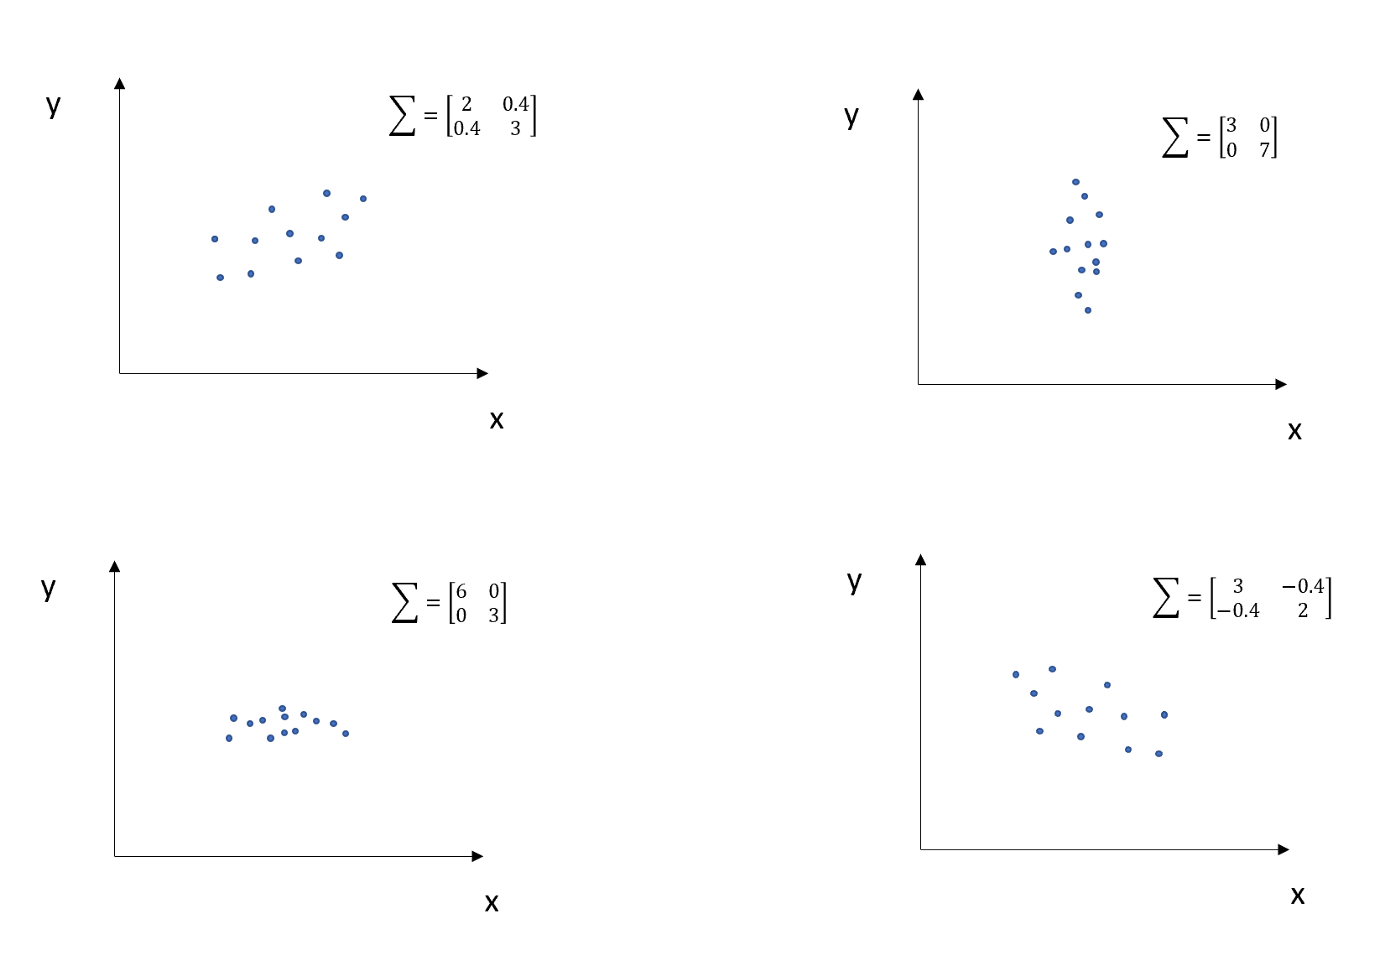
\includegraphics[width=4in]{img/covariance} 
\end{figure}
\end{frame}


\begin{frame}
\frametitle{Application: Principal Component Analysis}
\begin{small}
To this matrix $\Sigma$ we assign two elements: a \textcolor{blue}{vector} that will point into the direction of the larger spread of data and a \textcolor{blue}{number} equal to the spread (variance) of that direction. These two elements are, respectively, an \textcolor{blue}{Eigenvector} and \textcolor{blue}{Eigenvalue} of  $\Sigma$.
If we sort our eigenvectors in \textcolor{blue}{descending order} with respect to their eigenvalues, we will have that the first eigenvector accounts for the largest spread among data, and so forth (under the condition that all these new directions, which describe a new space, are orthogonal among each other).
\end{small}
\begin{figure}
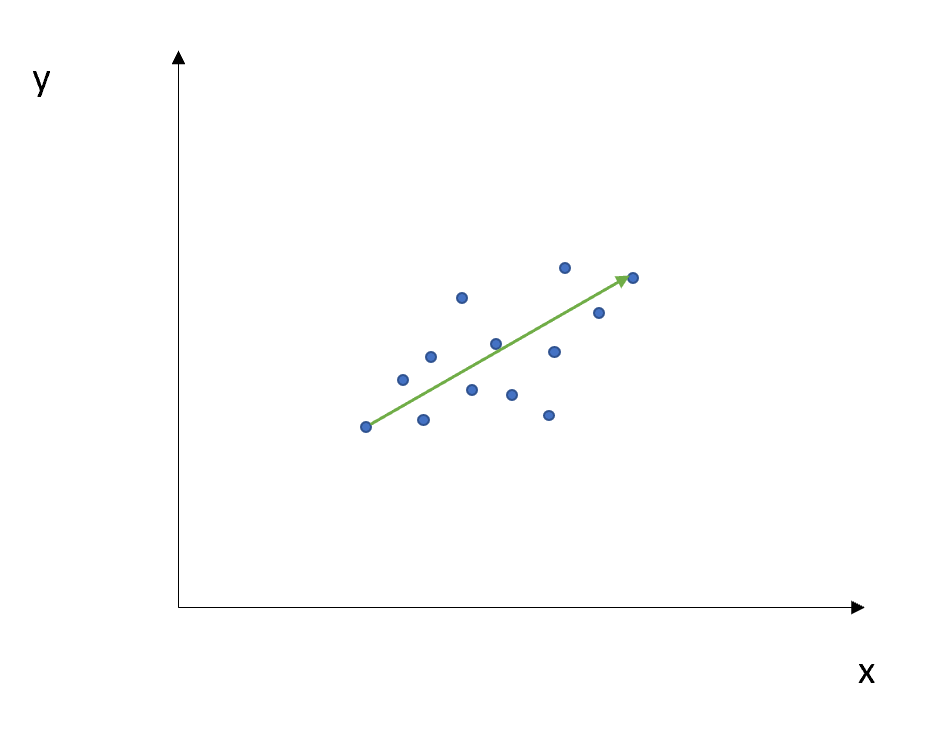
\includegraphics[width=2in]{img/eigenvalue} 
\end{figure}
\end{frame}


\begin{frame}
\frametitle{Numerical Example (PCA)}
\begin{small}
\begin{figure}
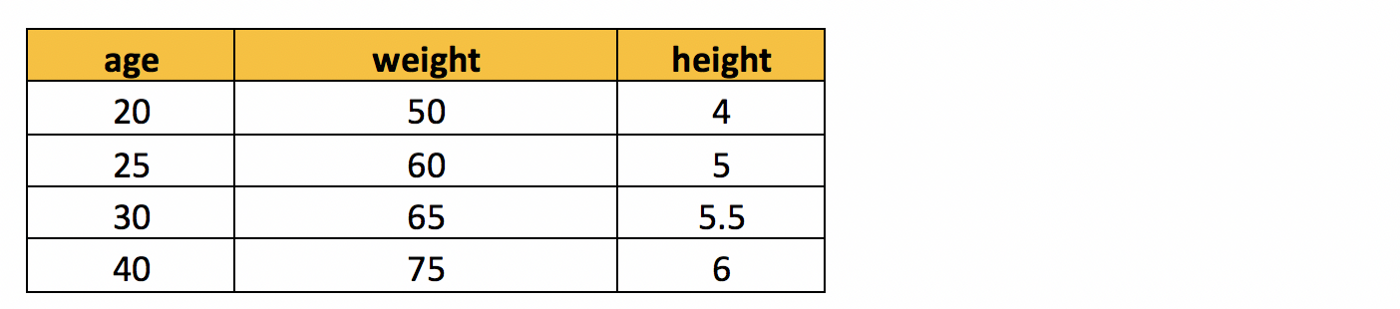
\includegraphics[width=3in]{img/table} 
\end{figure}
Covariance matrix:
$$\begin{pmatrix}
72.9&87.5&6.875  \\
87.5&108.3&8.75 \\
6.875&8.75&0.73
\end{pmatrix}$$

Eigenvectors (PCA components)
$$\begin{pmatrix}
0.63&0.77&0.06 \\
0.77&-0.617&-0.16 \\
0.08&-0.148&0.98
\end{pmatrix}$$

Eigenvalues (explained variances of the  components)
$$
(180, 1.38, 0.005)
$$

\end{small}
\end{frame}


\begin{frame}
\frametitle{Numerical  Example (PCA)}
\begin{small}
If there are eigenvalues \textcolor{blue}{close to zero}, they represent components that may be \textcolor{blue}{discarded}.
\vskip 10pt
 We can compute  the \textcolor{blue}{explained variance ratio of the first component} which is $0.99$, that is, the first component is enough to explain up to $99\%$ variance in the data. 
\vskip 10pt
We can now project our data into a $4x1$ matrix instead of a $4x3$ matrix, thereby reducing the dimension of the variables, with a minor loss in information.
\vskip 10pt
This is done multiplying the  data matrix with the eigenvector
$$\begin{pmatrix}
20&50&4  \\
25&60&5 \\
30&65&5.5 \\
40&75&6
\end{pmatrix}
\begin{pmatrix}
0.63\\
0.77\\
0.08
\end{pmatrix}=\begin{pmatrix}
51.42  \\
62.35 \\
69.39\\
83.43
\end{pmatrix}
$$
\begin{tiny}This can be seen  as a linear regression where  the  regression coefficients are the  components of the eigenvectors\end{tiny}

\end{small}
\end{frame}


\begin{frame}
\frametitle{Quadratic forms}
\begin{small}
A \textcolor{blue}{quadratic form}  is a function $Q:\R^n \rightarrow \R$ of the form
$$
Q({\bf x})={\bf x}^{\rm T} A {\bf x}= \sum_{i,j=1}^n a_{ij} x_i x_j,
$$ 
where $A=(a_{ij})$ is a $n \times n$ \textcolor{blue}{symmetric matrix} and ${\bf x}'=(x_1,\ldots,x_n)$ is a vector in $\R^n$.
\vskip 10pt
\textcolor{blue}{Remark:} Since the  coefficient of $x_ix_j$ is $a_{ij}+a_{ji}$, the quadratic form doesn't change
if we replace both coefficients by $\frac{a_{ij}+a_{ji}}{2}$, which corresponds to assume that $A$ is \textcolor{blue}{symmetric}.
\vskip 10pt
\textcolor{blue}{Example:} Both matrices  
$$\begin{pmatrix}
1&2 \\
3&4
\end{pmatrix} \quad \text{ and } \quad \begin{pmatrix}
1& 5/2 \\
5/2& 4
\end{pmatrix}$$
have the same  quadratic form $Q(x,y)=x^2+4y^2+5xy$.

\begin{tiny}For each  quadratic form there exists  a unique symmetric matrix \end{tiny}

\end{small}
\end{frame}

\begin{frame}
\frametitle{Quadratic forms and their sign}
\begin{small}
A $n \times n$ \textcolor{blue}{symmetric} matrix is said to be :
\begin{enumerate}
\item \textcolor{blue}{Positive definite} if
$
{\bf x}' A {\bf x}>0,
$ 
for all ${\bf x} \neq {\bf 0}$.

\item \textcolor{blue}{Negative definite} if ${\bf x}' A {\bf x}<0$ for all ${\bf x} \neq {\bf 0}$.

\item \textcolor{blue}{Positive semi-definite} if ${\bf x}' A {\bf x}\geq0$ for all ${\bf x} \in \R^n$.

\item \textcolor{blue}{Negative semi-definite} if ${\bf x}' A {\bf x}\leq0$ for all ${\bf x} \in \R^n$.

\item \textcolor{blue}{Indefinite} if both $
{\bf x}' A {\bf x}>0
$ and $
{\bf x}' A {\bf x}<0
$ are possible.
\end{enumerate}
\vskip 12pt
\textcolor{blue}{Example:}
$$
{\bf x}' A {\bf x}=(x,y) \begin{pmatrix} 1 & -1 \\ -1 & 1 \end{pmatrix}
\begin{pmatrix} x \\ y \end{pmatrix}=(x-y)^2 \geq 0
$$
Therefore, $A$ is positive semi-definite.
\end{small}
\end{frame}

\begin{frame}
\frametitle{Quadratic forms and their sign}
\begin{small}
\textcolor{blue}{Theorem:} Let A a $n \times n$ \textcolor{blue}{symmetric} matrix.
Then:
\begin{enumerate}
\item $A$ is \textcolor{blue}{positive definite} $\Longleftrightarrow$ all eigenvalues of $A$ are $>0$.

\item $A$ is \textcolor{blue}{negative definite} $\Longleftrightarrow$  all eigenvalues of $A$ are $<0$.
\item $A$ is \textcolor{blue}{positive semi-definite} $\Longleftrightarrow$ all eigenvalues of $A$ are $\geq0$.
\item $A$ is \textcolor{blue}{negative semi-definite} $\Longleftrightarrow$  all eigenvalues of $A$ are $ \leq0$.
	\item$A$ is \textcolor{blue}{indefinite} $\Longleftrightarrow$  $A$ has two eigenvalues of different sign.
\end{enumerate}
\vskip 12pt
\textcolor{blue}{Example:}
The eigenvalues of $A=\begin{pmatrix} 1 & -1 \\ -1 & 1 \end{pmatrix}$ are $\lambda_1=0$ and $\lambda_2=2$ since  $P(\lambda)=\lambda(\lambda-2)$.


\end{small}
\end{frame}\begin{frame}
\frametitle{Quadratic forms and their sign}
\begin{small}
Let $A$ be a $n \times n $ matrix. The \textcolor{blue}{principal minors}  are the determinants $\Delta_k$ obtained crossing out the same $n-k$ columns and rows of $A$. The \textcolor{blue}{leading principal minors}  are the determinants $D_k$ obtained crossing out the last $n-k$ columns and rows of $A$.
\vskip 10pt
\textcolor{blue}{Theorem:} Let A a $n \times n$ \textcolor{blue}{symmetric} matrix.
Then:
\begin{enumerate}
\item $A$ is \textcolor{blue}{positive definite} $\Longleftrightarrow$ $D_k>0$ for all $k=1,...,n$.

\item $A$ is \textcolor{blue}{negative definite} $\Longleftrightarrow$ $(-1)^k D_k>0$ for all $k=1,...,n$.

\item If $A$ is \textcolor{blue}{positive semi-definite} $\Longleftrightarrow$ $\Delta_k\geq 0$ for all $k=1,...,n$.

\item If $A$ is \textcolor{blue}{negative semi-definite} $\Longleftrightarrow$ $(-1)^k \Delta _k\geq 0$ for all $k=1,...,n$.

\item If none of the above conditions hold then $A$ is \textcolor{blue}{indefinite}.
\end{enumerate}
 \textcolor{blue}{Example:}
$$A=\begin{pmatrix} -3 & 2 & 0 \\ 2 & -3 & 0 \\ 0& 0 & -5\end{pmatrix}$$
Since $D_1=-3$, $D_2=5$, and $D_3=-25$, $A$ is negative definite.


\end{small}
\end{frame}

\begin{frame}
\frametitle{Examples}
\begin{small}
\begin{enumerate}
\item Consider the matrix $$A=\begin{pmatrix} 1 & 4 & 6 \\ 4 & 2 & 1 \\ 6& 1 & 6\end{pmatrix}$$
Since $D_1=1$, $D_2=-14$, and $D_3=-109$, we get that none of the conditions hold, thus the matrix is \textcolor{blue}{indefinite}.

\item Consider the matrix $$A=\begin{pmatrix} 3 & -1 & 0 \\ -1 & 2 & -1 \\ 0& -1 & 3\end{pmatrix}$$
Since $D_1=3$, $D_2=5$ and $D_3=12$ it is \textcolor{blue}{positive definite}.

\item The symmetric matrix associated to the quadratic form $xy+yz$ is \textcolor{blue}{indefinite}
since $D_1=D_3=0$ and $D_2=-\frac{1}{4}$.
\end{enumerate}

\end{small}
\end{frame}
\end{document}
\begin{frame}
\frametitle{Chapter 11: Functions of several variables}
\begin{small}
\begin{itemize}

\item In many economic applications, we have to deal with situations where several variables have to be included in the mathematical model. 

\item \textcolor{blue}{Example}: The Cobb-Douglas production function applied to an agricultural production gives the number of units produced depending on the capital invested, the labour and the area of land used for the production.

\item \textcolor{blue}{Read} Sections 11.3 (Total differential), 11.5 (Partial rate of change and elasticity; homogeneous functions), 11.6 (Implicit functions), 11.8 (Constrained optimization), 11.9 (Double integrals), and Chapter 12 (Differential and difference equations)

\item \textcolor{blue}{Exercises:} 11.11 a), 11.21, 11.22
\end{itemize}

\end{small}
\end{frame}



\begin{frame}
\frametitle{11.1 Preliminaries}
\begin{small}
\begin{itemize}
\item A \textcolor{blue}{function of several variables} is a map $f: D_f \rightarrow \R$ where $D_f \subset \R^n$, and for any variable ${\bf x}=(x_1,\dots,x_n)\in D_f$ it assigns a number
$f({\bf x})=f(x_1,\dots,x_n)$.

\item If $n=2$, the graph of $f$ with $z=f(x,y)$ is called a \textcolor{blue}{surface} and it is plotted in $\R^3$.

\item If $n=2$ a \textcolor{blue}{level curve} of $f$ is a curve in $\R^2$ given by $$z=f(x,y)=C.$$

\item A function $f:D_f \subset \R^n \rightarrow \R$ is said to be \textcolor{blue}{continuous}
at ${\bf x}_0 \in D_f$ if $$\lim_{{\bf x} \rightarrow {\bf x}_0} f({\bf x})=f({\bf x}_0),$$ that is, for any sequence ${\bf x}_n$ in $\R^n$ convergent to ${\bf x}_0$,
the sequence $f({\bf x}_n)$ converges to $f({\bf x}_0)$, that is, for any $\epsilon>0$ there exists $\delta>0$ such that
$\vert f({\bf x})-f({\bf x}_0) \vert<\epsilon$ provided $\vert {\bf x}-{\bf x_0} \vert <\delta$.
\end{itemize}

\end{small}
\end{frame}\begin{frame}
\frametitle{1.2 Partial derivatives; gradient}
\begin{small}
\begin{itemize}
\item Intervals $(a,b)$ in $\R$ are replaced by $\epsilon$-neighbourhood $U_{\epsilon}({\bf x}_0)$, which is the open ball of center ${\bf x}_0$ and radius $\epsilon$ in $\R^n$, that is,
$$
U_{\epsilon}({\bf x}_0)=\left\{ {\bf x} \in \R^n: \vert {\bf x}-{\bf x}_0 \vert < \epsilon \right\}.
$$
\item  A function $f: D_f \subset\R^2 \rightarrow \R$ defined on a neighborhood of ${\bf x}_0=(x_0,y_0)$ is \textcolor{blue}{partially differentiable} with respect to $x$ at ${\bf x}_0$ if the limit
$$
\lim_{h\rightarrow 0} \frac{f(x_0+h,y_0)-f(x_0,y_0)}{h} \qquad \text{exists},
$$
and is \textcolor{blue}{partially differentiable} with respect to $y$ at ${\bf x}_0$ if the limit
$$
\lim_{h\rightarrow 0} \frac{f(x_0,y_0+h)-f(x_0,y_0)}{h} \qquad \text{exists}.
$$
\item Both limits are denoted the partial derivative of $f$ with respect to $x$ and $y$ at ${\bf x}_0$ and denoted $f_x({\bf x}_0)$, $f_y({\bf x}_0)$ or 
$\frac{\partial f({\bf x}_0)}{\partial x} $, $\frac{\partial f({\bf x}_0)}{\partial y}$.


\end{itemize}

\end{small}
\end{frame}

\begin{frame}
\frametitle{1.2 Partial derivatives; gradient}
\begin{small}
\begin{itemize}
\item \textcolor{blue}{Geometric interpretation:} $f_x({\bf x}_0)=$ ($f_y({\bf x}_0)$) slope of the tangent line $f_T(x)$ to the curve of intersection of the surface $z=f(x,y)$ and the plane $y=y_0$ ($x=x_0$) at point $(x_0,y_0,z_0)$.

\item Both tangent lines $f_T(x)$ and $f_T(y)$ span a plane $f_T(x,y)$ which is called the \textcolor{blue}{tangent plane} to $z=f(x,y)$ at point ${\bf x}_0$, and the equation of the tangent plane is
$$
f_T(x,y)=f(x_0,y_0)+f_x(x_0, y_0) (x-x_0) +f_y(x_0, y_0) (y-y_0).
$$

\item \textcolor{blue}{Example:} Total cost of a firm producing $x$ units of product $A$ and $y$ units of product $B$ is
$$
C(x,y)=200+22x+16y^{3/2}.
$$ 
Marginal costs: $C_x(x,y)=22, C_y(x,y)=24 \sqrt{y}$.

\item We can consider \textcolor{blue}{higher-order partial derivatives} of $f:D_f \subset \R^n \rightarrow \R$, when they exists. For example
$$
f_{xy}(x,y)=\frac{\partial}{\partial y} \left( \frac{\partial f(x,y)}{\partial x}\right)=
\frac{\partial^2 f(x,y)}{\partial y \partial x}.
$$ 
\end{itemize}

\end{small}
\end{frame}

\begin{frame}
\frametitle{1.2 Partial derivatives; gradient}
\begin{small}
\begin{itemize}


\item \textcolor{blue}{Theorem (Young):} If $f_{xy}$ and $f_{yx}$ are continuous, they coincide.

\item \textcolor{blue}{Example:} $f(x,y)=\sin(3x-y)$, $f_{xy}=f_{yx}=3 \sin(3x-y)$.

\item If $f:D_f \subset \R^n \rightarrow \R$ is partially differentiable at ${\bf x}_0 \in D_f$, the vector
$$
{\bf grad}f({\bf x}_0)=(f_{x_1}({\bf x}_0),\dots,f_{x_n}({\bf x}_0))^{\rm T}
$$
is called the \textcolor{blue}{gradient} of $f$ at ${\bf x}_0$. 

\item The gradient gives the direction which the function $f$ at point ${\bf x}_0$ increases the most.

\item \textcolor{blue}{Example:} $f(x,y)=2x^2+\frac12 y^2$, ${\bf grad}f(1,2)=(4, 2)^{\rm T}$ 

\item The gradient of $f$ at ${\bf x}_0$ is orthogonal to the tangent line to the level curve at point this point.

\item \textcolor{blue}{Example:} production function: $f(x,y)=3x^2y+0.5 x e^y$, $x=$labour, $y=$capital

${\bf grad}f(10,\ln 12)=(155.09, 360)^{\rm T}$, so to increase at maximum the production, the firm should increase labour and capital in the ratio $155.09:360$
\end{itemize}

\end{small}
\end{frame}


\begin{frame}
\frametitle{10.4 Generalized chain rule: directional derivatives}
\begin{small}
\begin{itemize}
\item Let $f:D_f \subset \R^n \rightarrow \R$ be continuously partially differentiable, and let ${\bf r}$ be a unit vector in $\R^n$. The \textcolor{blue}{directional derivative} of $f$ at point ${\bf x}_0 \in D_f$ in the direction ${\bf r}$ is defined as
$$
\frac{\partial f}{\partial {\bf r}} ({\bf x}_0)={\bf grad} f ({\bf x}_0)^{\rm T} \cdot {\bf r}.
$$

\item The partial derivatives are special directional derivatives, when ${\bf r}$ are the elements of the standard basis.


\item  The directional derivative gives the approximate change of the function if we move one unit from ${\bf x}_0$ in the direction ${\bf r}$. 


\item \textcolor{blue}{Example:} cost function of a firm producing 3 goods: $f(x,y,z)=20+x^2+2y+3z+2xz$

${\bf grad}f(10,15,20)=(60,2,23)^{\rm T}$, 
$
\frac{\partial f}{\partial (1,2,2)} (10,15,20)=\frac{110}{3}.
$

If we increase the production of good 1 by 1, and of goods 2 and 3 by 2 the cost increases by $3 \frac{110}{3}=110$.
\end{itemize}

\end{small}
\end{frame}

\begin{frame}
\frametitle{11.7 Unconstrained optimization}
\begin{small}
\begin{itemize}
\item A function $f:D_f \subset \R^n \rightarrow \R$ has a \textcolor{blue}{local maximum} (\textcolor{blue}{minimum})
at ${\bf x}_0$ if there exists an $\epsilon$-neighbourhood $U_{\epsilon}({\bf x}_0)\in D_f$ such that
$$
f({\bf x}) \leq f({\bf x}_0) \qquad (f({\bf x}) \geq f({\bf x}_0) )
$$
for all ${\bf x} \in U_{\epsilon}({\bf x}_0)$. If the inequality holds for all ${\bf x} \in D_f$, we say it is a global maximum (minimum).

\item \textcolor{blue}{Theorem (Necessary 1st order condition):} If $f$ has a local maximum or minimum at ${\bf x}_0$ then ${\bf grad} f ({\bf x}_0)={\bf 0}$.

\item Points ${\bf x}_0$ that ${\bf grad} f ({\bf x}_0)={\bf 0}$ are called \textcolor{blue}{stationary points}. 

\item Stationary points that are neither a local maximum or minimum are called \textcolor{blue}{saddle points}.


\end{itemize}

\end{small}
\end{frame}

\begin{frame}
\frametitle{11.7.1 Optimality conditions}
\begin{figure}
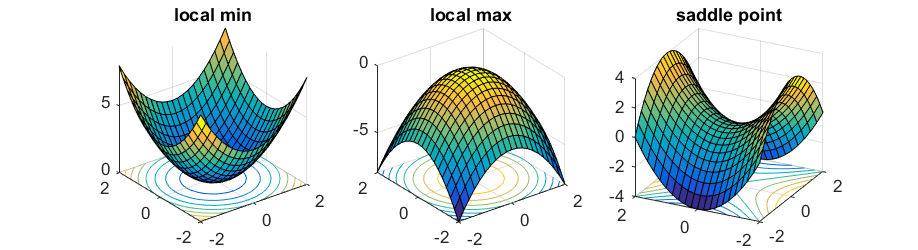
\includegraphics[width=5in]{img/minmaxsaddle.png} 
\end{figure}
\end{frame}

\begin{frame}
\frametitle{11.7.1 Optimality conditions}
\begin{small}
\begin{itemize}

\item \textcolor{blue}{The Hessian matrix} of a twice continuously partially differentiable function $f: D_f \subset\R^n \rightarrow \R$ at a point ${\bf x}_0$ is the matrix:
$$
H_f({\bf x}_0)=\left(f_{x_i x_j}({\bf x}_0)\right)_{1 \leq i,j \leq n}.
$$


\item \textcolor{blue}{Theorem (Sufficient 2nd order condition):} Let ${\bf x}_0$ be a stationary point of $f$. Then:
\begin{enumerate}
\item If $H_f({\bf x}_0)$ is negative (positive) definite, then ${\bf x}_0$ is a local
maximum (minimum) 
\item If $H_f({\bf x}_0)$ is indefinite, then ${\bf x}_0$ is a saddle point.
\item If $H_f({\bf x})$ is negative (positive) definite for all ${\bf x} \in D_f$, then ${\bf x}_0$ is a global
maximum (minimum). 
\end{enumerate}

\item \textcolor{blue}{Theorem ($n=2$):} Let ${\bf x}_0$ be a stationary point of $f$. Then:
\begin{enumerate}
\item If $\vert H_f({\bf x}_0)\vert >0$, then:
\begin{itemize}
\item If $f_{xx}({\bf x}_0)<0$ or $f_{yy}({\bf x}_0)<0$, then ${\bf x}_0$ is a local maximum.
\item If $f_{xx}({\bf x}_0)>0$ or $f_{yy}({\bf x}_0)>0$, then ${\bf x}_0$ is a local minimum.
\end{itemize}
\item If $\vert H_f({\bf x}_0)\vert <0$, then ${\bf x}_0$ is a saddle point.
\item  If $\vert H_f({\bf x}_0) \vert =0$, we don't know.
\end{enumerate}

\end{itemize}

\end{small}
\end{frame}





\begin{frame}
\frametitle{11.7.1 Optimality conditions}
\begin{small}
\begin{itemize}
\item \textcolor{blue}{Example:} A firm can sell each piece of product $X/Y$ for $45/55$ euros. The revenue is $R(x,y)=45x+55y$. The production cost is
$$
C(x,y)=300+x^2+1.5 y^2-25 x- 35 y.$$ 
The total profit is
$$
f(x,y)=R(x,y)-C(x,y).
$$
We want to know the maximum profit the firm can make. We first find the stationary points of $f$:
$$
f_x=-2x+70=0, \; \; f_y=-3y+90=0 \quad \Longrightarrow {\bf x}_0=(35,30).
$$
We next check the 2nd order conditions:
since $H_f({\bf x})$ is negative definite for all ${\bf x}$, ${\bf x}_0$ is a global maximum of $f$. The maximal profit is $f(35,30)=2,275$.

\end{itemize}

\end{small}
\end{frame}

\begin{frame}
\frametitle{11.7.2 Method of least squares}
\begin{small}
\begin{itemize}
\item Consider a linear system $A {\bf x}={\bf b}$ that has \textcolor{blue}{no solution}.

\item We want to find a vector ${\bf e}$ with minimal $\vert {\bf e} \vert$ and such that the system
$$
A {\bf x}+{\bf e}={\bf b}
$$
has a solution.
In this case, a solution ${\bf x}$ is called \textcolor{blue}{a least square solution}.

\item This is equivalent to find the \textcolor{blue}{orthogonal projection} of {\bf b} onto the subspace of all vectors $A {\bf x}$, that is, we want to find ${\bf x}^{\ast}$ that minimizes the distance $\vert A{\bf x}-{\bf b}\vert$ for all ${\bf x}$.

\item  The solution is ${\bf x}^{\ast}$ such that
$$
(A{\bf x}^{\ast}-{\bf b})^{\rm T} \cdot  (A{\bf x})=0, \quad \text{ for all } {\bf x}.
$$


\item This is equivalent to solve the linear system of equations
$$
A^{\rm T} {\bf b}= A^{\rm T}  A {\bf x}^{\ast}.
$$
\end{itemize}

\end{small}
\end{frame}\begin{frame}
\frametitle{11.7.2 Method of least squares}
\begin{small}
\begin{itemize}
\item Assume that we have $n$ \textcolor{blue}{measurements}
${\bf x}=(x_1,...,x_n)$ and ${\bf y}=(y_1,...,y_n)$ of two variables $x$ and $y$, respectively.

\item We want to find the line $y=ax+b$ that describes the relation between both variables using the least square approximation.

\item Here $A$ is the $n \times 2$ matrix of the observations ${\bf x}$ and a column of ones, ${\bf b}$ is the vector ${\bf y}$, and the least square solution is $(a,b)^{\rm T}$.

\item In this case, the solution to the system $
A^{\rm T} {\bf b}= A^{\rm T}  A {\bf x}^{\ast}
$ is
\begin{equation*} \begin{split}
a&=\frac{n \sum_{i=1}^n x_i y_i-\left(\sum_{i=1}^n x_i\right) \left( \sum_{i=1}^n y_i\right)}{n \sum_{i=1}^n x_i^2-\left( \sum_{i=1}^n x_i\right)^2} \\
b&=\frac{\sum_{i=1}^n y_i-a \sum_{i=1}^n x_i}{n}
\end{split}
\end{equation*}
\end{itemize}

\end{small}
\end{frame}
\end{document}

